\documentclass[letterpaper]{article}  

\usepackage{graphicx}
\usepackage{float}
\usepackage[margin=0.5in]{geometry}
\usepackage{caption}
\usepackage{subcaption}


\begin{document}


\title{STA511 Homework \#1}
\date{September 30, 2015}
\author{Abbas Rizvi}
\maketitle

\begin{enumerate}

\item No work required for question 1

\item My answer to \# 2, has multiple parts.

\begin{enumerate}
\item X is a uniform random variable $(X$ $\sim$ $U(0,1))$. The histogram is shown in Figure 1.
\begin{figure}[htpb]
\centering
\caption{(Left panel): Random Sample 1. (Right panel): Random Sample 2 }
\centering

\includegraphics[scale=0.6]{hw1-q2a-runiform-histogram.pdf}
\end{figure}

\item Here's my code for part a
\begin{verbatim}
#part 2a-1
runif.histogram <- runif(1000,0,1)

#part 2a-2
x <- runif.histogram
y <- 3.14*x + 3.14/4


pdf("hw1-q2a-runiform-histogram.pdf")
par(mfrow=c(1,2),bg="gray")
hist(runif.histogram, main="X ~ U(0,1) Simulations", xlab = 'X')
hist(y, main="Y = pi/X - (pi/4) Simulations", xlab = 'Y = pi/X - (pi/4)')
dev.off()
\end{verbatim}

\item Here are my X + Z results

\begin{figure}
    \centering
    \begin{subfigure}{0.4\textwidth}
        \centering
        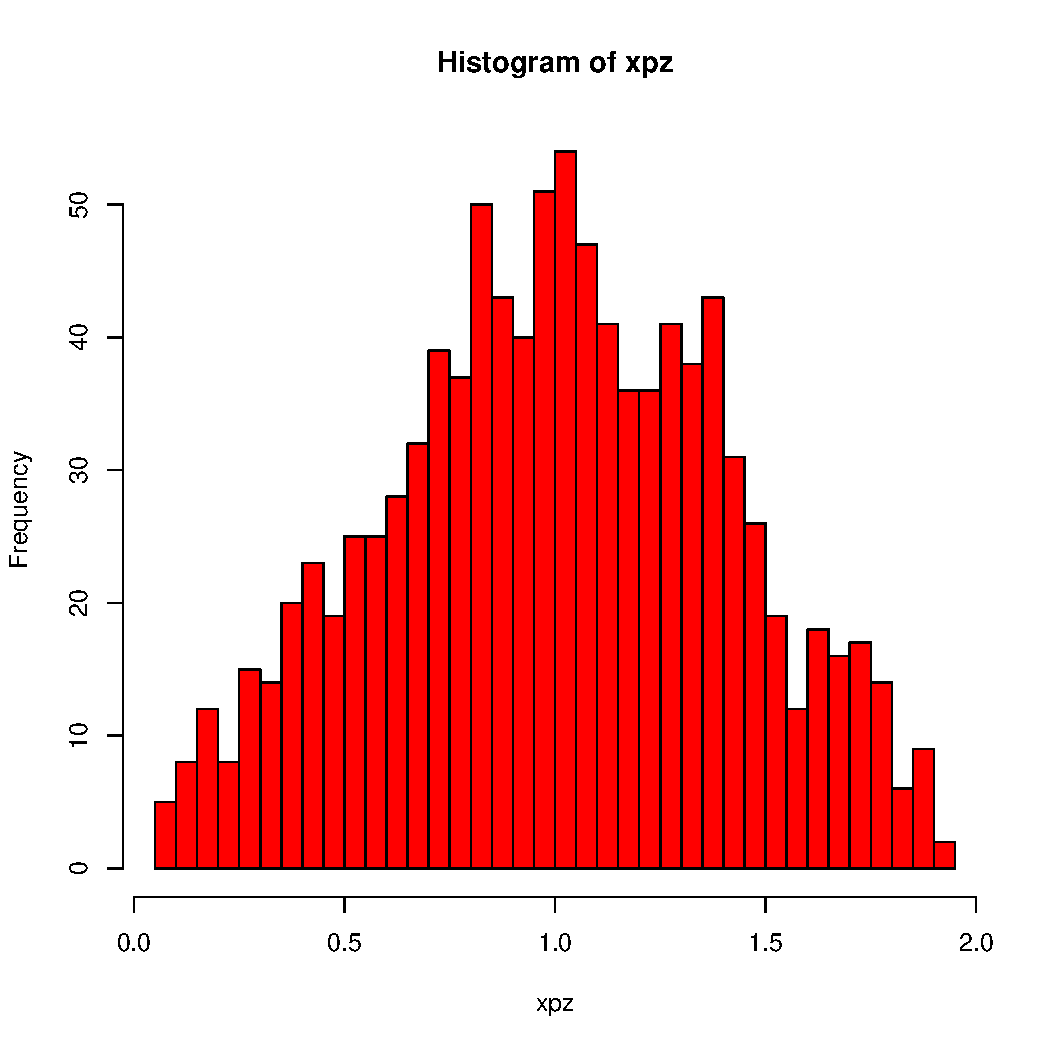
\includegraphics[width=\textwidth]{hw1-q2c-xpz.pdf}
        \caption{$X + Z$}
    \end{subfigure}
    \begin{subfigure}{0.4\textwidth}
        \centering
        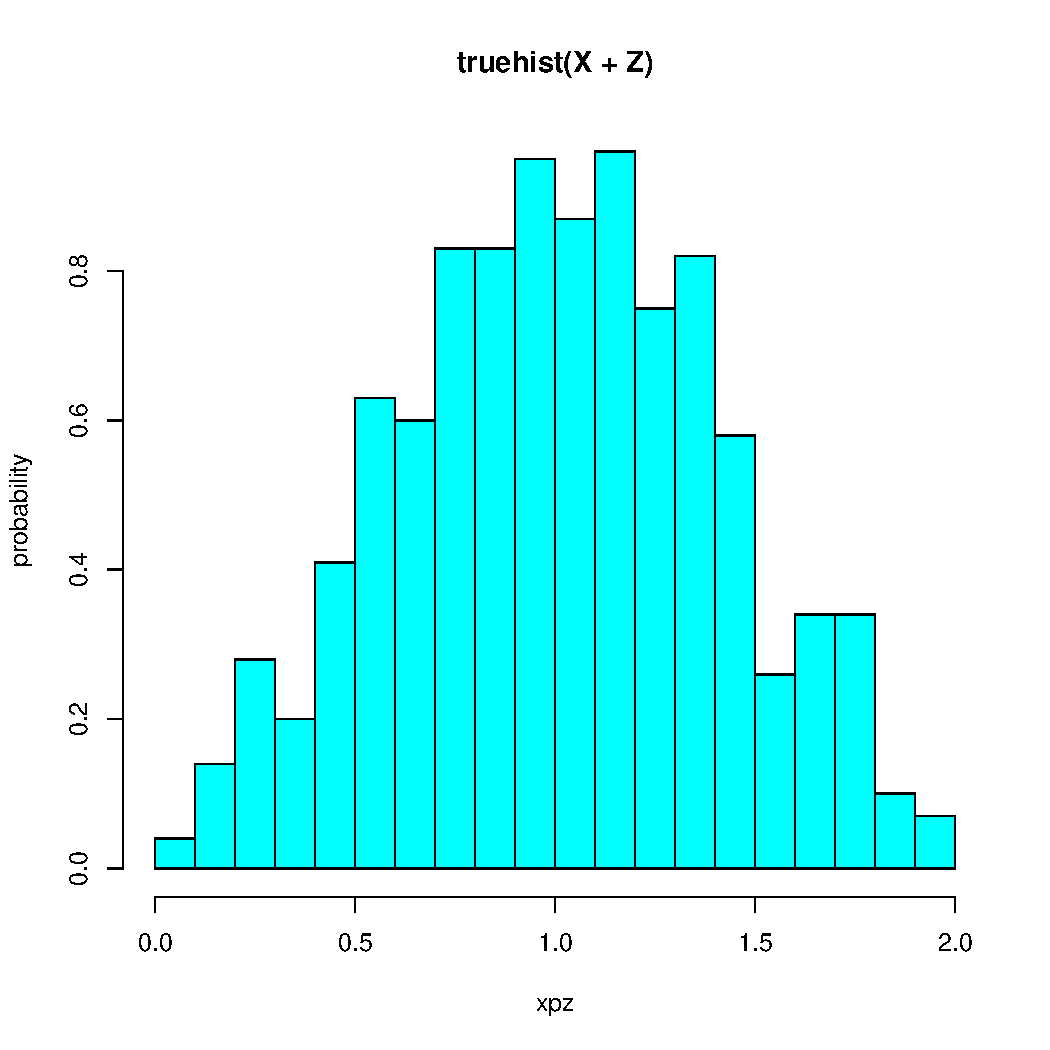
\includegraphics[width=\textwidth]{hw1q2d-truehist.pdf}
        \caption{$X + Z$ truehist$()$}
    \end{subfigure}
\end{figure}

Here is my code for part 2b:
\begin{verbatim}
z <- runif(1000,0,1)
xpz <- x + z
pdf("hw1-q2c-xpz.pdf")
par(bg="gray")
hist(xpz)
dev.off()
\end{verbatim}

\end{enumerate} 

\item My randomly assigned grades to class roster with correspoding letter grade.

\begin{table}[ht]
\centering
\begin{tabular}{rlllrl}
  \hline
 & Name & Program.and.Plan & Level & Percent.Grade & Letter.Grade \\ 
  \hline
1 & An,Bo & Pharmaceutcl Sci Doctoral  & Doctoral 2 & 73.00 & C \\ 
  2 & Bu,Yahao & Public Health Masters  & Masters 2 & 68.54 & C \\ 
  3 & Chang,Huiru & Public Health Masters  & Masters 2 & 63.61 & C \\ 
  4 & Chen,Jiangwang & Public Health Masters  & Masters 2 & 71.97 & C \\ 
  5 & Eum,Youngseob & Arts \& Sciences Doctoral  & Doctoral 1 & 74.52 & C \\ 
  6 & Ganley,Kevin & Public Health Masters  & Masters 1 & 67.26 & C \\ 
  7 & Hess,Katelyn & Arts \& Sciences Masters  & Masters 1 & 84.34 & B \\ 
  8 & Hsu,En-Shuo & Public Health Masters  & Masters 1 & 80.25 & B \\ 
  9 & Jai Kumar Ahuja,Suruchi & Public Health Masters  & Masters 1 & 82.86 & B \\ 
  10 & Jin,Yuxuan & Public Health Doctoral  & Doctoral 1 & 79.65 & B- \\ 
  11 & Karaesmen,Ezgi & Roswell Park Doctoral  & Doctoral 2 & 76.51 & B- \\ 
  12 & Krishnan,Krithika & Public Health Masters  & Masters 1 & 89.05 & B+ \\ 
  13 & Lin,Jieya & Public Health Masters  & Masters 1 & 95.36 & A \\ 
  14 & Mandava,Aishwarya & Public Health Masters  & Masters 1 & 99.15 & A \\ 
  15 & Marsales,Harry & Public Health Masters  & Masters 2 & 68.66 & C \\ 
  16 & Morrell,Kayla & Public Health Masters  & Masters 1 & 83.43 & B \\ 
  17 & Niu,Jin & Pharmaceutcl Sci Doctoral  & Doctoral 2 & 91.37 & A- \\ 
  18 & Rizvi,Abbas & Roswell Park Doctoral  & Doctoral 2 & 92.22 & A- \\ 
  19 & Rosario,Spencer Rae & Roswell Park Doctoral  & Doctoral 2 & 84.09 & B \\ 
  20 & Schiller,Emily & Public Health Masters  & Masters 1 & 99.41 & A \\ 
  21 & Song,Jiaming & Public Health Masters  & Masters 1 & 87.51 & B+ \\ 
  22 & Spencer,Mary & Public Health Masters  & Masters 1 & 65.71 & C \\ 
  23 & Sun,Xiaoxi & Public Health Masters  & Masters 1 & 97.25 & A \\ 
  24 & Tanue,Terence Wankah & Public Health Masters  & Masters 1 & 69.08 & C \\ 
  25 & Tian,Mingmei & Public Health Masters  & Masters 2 & 63.18 & C \\ 
  26 & Vucic,Luther & Public Health Masters  & Masters 1 & 78.60 & B- \\ 
  27 & Wackeroth,Wolf Michael & Public Health Masters  & Masters 1 & 68.49 & C \\ 
  28 & Wang,Jiefei & Public Health Masters  & Masters 1 & 93.77 & A- \\ 
  29 & Wang,Xue & Roswell Park Doctoral  & Doctoral 2 & 89.14 & B+ \\ 
  30 & Wu,Yin & Grad Sch of Ed Doctoral  & Doctoral 2 & 86.43 & B+ \\ 
  31 & Yang,Yang & Grad Sch of Ed Doctoral  & Doctoral 2 & 85.94 & B+ \\ 
  32 & Yang,Yujie & Pharmaceutcl Sci Doctoral  & Doctoral 2 & 81.69 & B \\ 
  33 & Yang,Zeyu & Public Health Masters  & Masters 1 & 63.28 & C \\ 
  34 & Yu,Xinyang & Biomedical Sci Doctoral  & Doctoral 2 & 78.93 & B- \\ 
  35 & Zhao,Yichen & Grad Sch of Ed Doctoral  & Doctoral 2 & 62.93 & C \\ 
   \hline
\end{tabular}
\end{table}

Here is my code:
\begin{verbatim}
#question 3
class.roster <- read.table("classlist.txt",sep="\t",header=TRUE)
Percent.Grade <- runif(35, 60, 100)
class.roster.2 <- cbind(class.roster, Percent.Grade)
class.roster.2 <- data.table(class.roster.2)

#remove weird -\xa0 symbol
class.roster.2$Program.and.Plan <- gsub("[-\xa0]", "",class.roster.2$Program.and.Plan)

library(data.table)
class.roster.2[Percent.Grade > 95, Letter.Grade := "A"]
class.roster.2[Percent.Grade >= 90 & Percent.Grade < 95, Letter.Grade := "A-"]
class.roster.2[Percent.Grade >= 85 & Percent.Grade < 90, Letter.Grade := "B+"]
class.roster.2[Percent.Grade >= 80 & Percent.Grade < 85, Letter.Grade := "B"]
class.roster.2[Percent.Grade >= 75 & Percent.Grade < 80, Letter.Grade := "B-"]
class.roster.2[Percent.Grade < 75, Letter.Grade := "C"]

install.packages('xtable')
library(xtable)

roster.table <- xtable(class.roster.2)
print(roster.table)

\end{verbatim}

\end{enumerate}

\end{document}
